\section{Expanding the Traffic Light System: Contexts and Refinement}
\label{tutorial_07}

\tick{\textbf{Goals:} We apply what we learned in the previous section by introducing a context with traffic light colors, and a refinement to integrate them. We will introduce another refinement for the push buttons.}

\subsection{Data Refinement}

We will continue the example from Section~\ref{tutorial_03}, where we built a simplified model of a traffic light controller.  The model was simplified because we abstracted the traffic lights to TRUE and FALSE, and a number of features were still missing.

We will introduce data refinement in this section.  The objective is to create a mapping between the abstract traffic light values and actual colors.  The following image depicts our mapping for the traffic light.

\begin{center}
	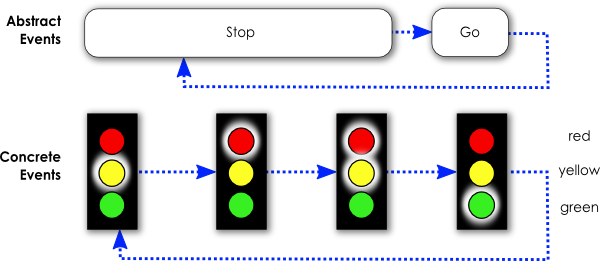
\includegraphics[width=0.60\textwidth]{img/tutorial/tl-colors.png}
	\label{fig:tl-colors}
\end{center}

For simplicity, the traffic light for pedestrians consists of only two lights, red and green.

We break this problem into two steps:

\begin{enumerate}
	\item Create a context with the data structures for the colors
	\item Create a refinement of the existing model that sees the new context and refines the boolean states into colors.
\end{enumerate}

\subsection{A Context with Colors}

Start by creating a context called \texttt{ctx1}, as described in Section~\ref{tutorial_05}.
We model the colors as constants:

\pencil{
\begin{description}
\CONSTANTS
	\begin{description}
		\Item{ red }
		\Item{ yellow }
		\Item{ green }
	\end{description}
\end{description}
}

These constants are part of a set:

\pencil{
\begin{description}
\SETS
	\begin{description}
		\Item{ COLORS }
	\end{description}
\end{description}
}

And last, we need to provide typing.  We do this by creating a partition (\ref{partition}):

\pencil{
\begin{description}
\AXIOMS
	\begin{description}
		\nItemX{ type }{ partition(COLORS, \{ red\} , \{ yellow\} , \{ green\} ) }
	\end{description}
\end{description}
}

\warning{Please note the curly braces \{\} around the colors.  It's very easy to forget these, which will result in typing errors that are very hard to interpret for a novice.
}

This completes the context.

\subsection{The Actual Data Refinement}


